\documentclass[11pt]{article}
\usepackage[T1]{fontenc}
\usepackage{lmodern,microtype,amsmath,amssymb,amsthm,mathtools,booktabs}
\usepackage[margin=1.05in]{geometry}
\usepackage{graphicx,tikz,placeins,needspace,float}
\usepackage[font=small,labelfont=bf]{caption}
\setlength{\intextsep}{9pt plus 2pt minus 2pt}
\setlength{\textfloatsep}{13pt plus 2pt minus 2pt}
% Original vector drawings. The three isometric unit vectors project to zero in sum.
\definecolor{boxink}{HTML}{223A41}
\definecolor{boxtop}{HTML}{F2D5A3}
\definecolor{boxleft}{HTML}{96BDB5}
\definecolor{boxright}{HTML}{5D9196}
\definecolor{boxgrid}{HTML}{B5C2C1}
\definecolor{boxwarm}{HTML}{E5B977}
\tikzset{boxface/.style={draw=boxink,line width=.46pt,line join=round}}

\newcommand{\TopTile}[3]{\filldraw[boxface,fill=boxtop]
  (#1,#2,#3) -- ++(1,0,0) -- ++(0,1,0) -- ++(-1,0,0) -- cycle;}
\newcommand{\XTile}[3]{\filldraw[boxface,fill=boxright]
  (#1,#2,#3) -- ++(0,1,0) -- ++(0,0,1) -- ++(0,-1,0) -- cycle;}
\newcommand{\YTile}[3]{\filldraw[boxface,fill=boxleft]
  (#1,#2,#3) -- ++(1,0,0) -- ++(0,0,1) -- ++(-1,0,0) -- cycle;}
\newcommand{\BoxOutline}{(0,0,4) -- (2,0,4) -- (2,0,0) --
  (2,2,0) -- (0,2,0) -- (0,2,4) -- cycle}

% Heights by row are (4,2) and (1,0).
\newcommand{\SevenCubes}{%
  \TopTile{0}{0}{4}\TopTile{1}{0}{2}\TopTile{0}{1}{1}
  \foreach \x/\y/\z in {2/0/0,2/0/1,1/0/2,1/0/3,1/1/0}{\XTile{\x}{\y}{\z}}
  \foreach \x/\y/\z in {0/2/0,0/1/1,0/1/2,0/1/3,1/1/0,1/1/1}{\YTile{\x}{\y}{\z}}}
\newcommand{\EmptyCornerFaces}{%
  \begingroup
  \colorlet{boxtop}{boxtop!20!white}
  \colorlet{boxleft}{boxleft!37!white}
  \colorlet{boxright}{boxright!37!white}
  \TopTile{1}{1}{0}
  \foreach \z in {1,2,3}{\XTile{0}{1}{\z}}
  \foreach \z in {2,3}{\YTile{1}{0}{\z}}
  \endgroup}

\newcommand{\StackAndTiling}{%
  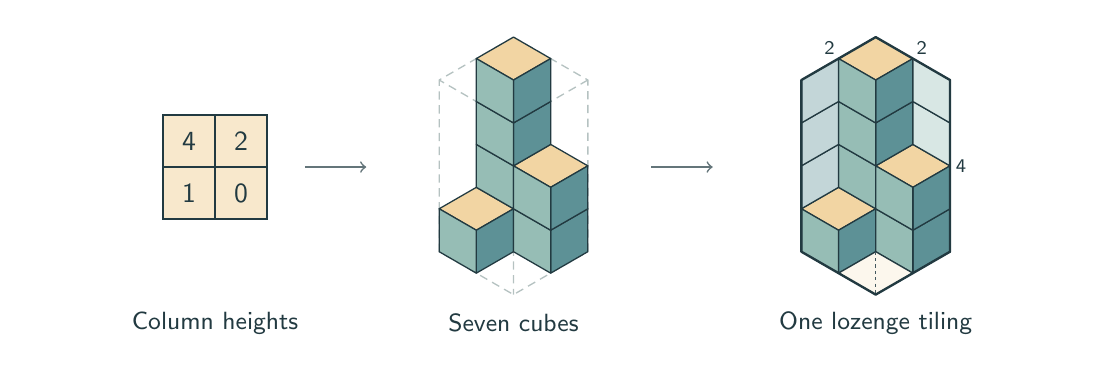
\begin{tikzpicture}[font=\sffamily\small,text=boxink]
    \path[use as bounding box] (-.12,-1.40) rectangle (13.05,2.52);
    \begin{scope}[shift={(1.60,.75)},x=.66cm,y=.66cm]
      \foreach \x/\y/\n in {0/0/4,1/0/2,0/-1/1,1/-1/0}{
        \draw[boxink,fill=boxtop!55,line width=.5pt] (\x,\y) rectangle ++(1,1);
        \node[font=\sffamily\normalsize] at ({\x+.5},{\y+.5}) {\n};}
    \end{scope}
    \draw[->,draw=boxink!70,line width=.6pt] (3.40,.75)--(4.18,.75);
    \begin{scope}[shift={(6.05,.22)},x={(.472cm,-.2725cm)},
                            y={(-.472cm,-.2725cm)},z={(0cm,.545cm)}]
      \draw[boxgrid,densely dashed,line width=.48pt] \BoxOutline;
      \draw[boxgrid,densely dashed,line width=.48pt]
        (2,0,0)--(0,0,0)--(0,2,0) (0,0,0)--(0,0,4)
        (2,0,4)--(2,2,4)--(0,2,4) (2,2,4)--(2,2,0);
      \SevenCubes
    \end{scope}
    \draw[->,draw=boxink!70,line width=.6pt] (7.80,.75)--(8.58,.75);
    \begin{scope}[shift={(10.65,.22)},x={(.472cm,-.2725cm)},
                            y={(-.472cm,-.2725cm)},z={(0cm,.545cm)}]
      \SevenCubes\EmptyCornerFaces
      \draw[draw=boxink!85,dash pattern=on 1.2pt off 1.1pt,line width=.42pt]
        (1,1,0)--(2,2,0);
      \draw[boxink,line width=.85pt,line join=round] \BoxOutline;
      \path (0,2,4)--(0,0,4) node[midway,above left,inner sep=1.2pt,font=\sffamily\scriptsize] {2};
      \path (0,0,4)--(2,0,4) node[midway,above right,inner sep=1.2pt,font=\sffamily\scriptsize] {2};
      \path (2,0,4)--(2,0,0) node[midway,right,inner sep=1.9pt,font=\sffamily\scriptsize] {4};
    \end{scope}
    \node at (2.26,-1.23) {Column heights};
    \node at (6.05,-1.23) {Seven cubes};
    \node at (10.65,-1.23) {One lozenge tiling};
  \end{tikzpicture}}

% One projected square. The angle is the first of its three rim vertices.
\newcommand{\UnitFaceInTiling}[2]{%
  \filldraw[draw=boxink,fill=#2,line width=.78pt]
    (0,0)--(#1:1)--({#1+60}:1)--({#1+120}:1)--cycle;
  \draw[draw=boxink!74,line width=.50pt,densely dotted]
    (0,0)--({#1+60}:1);}

% Left column: oblique physical views with the vertical axis upright.
% Right column: Figure 1's diagonal projection turned counterclockwise 90
% degrees. From the empty back corner the x,y,z rays have angles 60,300,180.
% The exposed edges at the opposite corner of the cube use the reverse rays.
\newcommand{\TwoUnitTilings}{%
  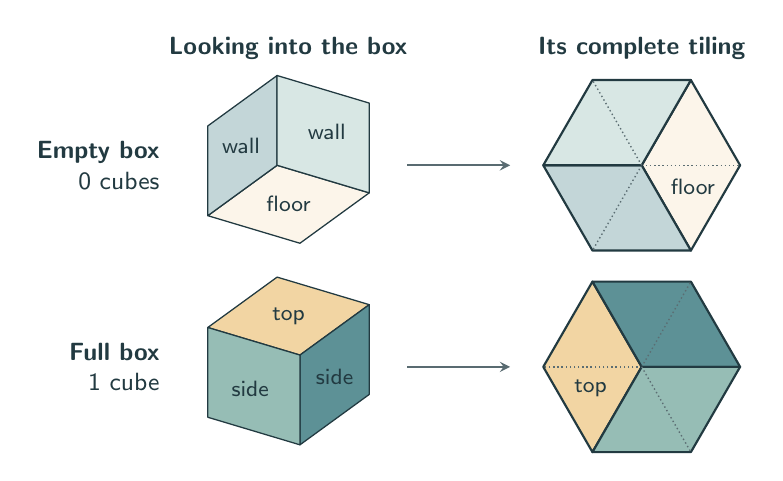
\begin{tikzpicture}[text=boxink,font=\sffamily\small,line join=round,>=stealth]
    \node[font=\sffamily\small\bfseries] at (.14,1.49) {Looking into the box};
    \node[font=\sffamily\small\bfseries] at (4.63,1.49) {Its complete tiling};
    \foreach \level/\offset/\stackname/\cubecount in
        {0/0/Empty box/0 cubes,1/-2.56/Full box/1 cube}{%
      \begin{scope}[shift={(0,\offset)}]
        \node[anchor=east,align=right] at (-1.37,0)
          {\textbf{\stackname}\\\cubecount};
        \begin{scope}[x={(1.17cm,-.35cm)},y={(-.88cm,-.64cm)},z={(0cm,1.14cm)},
            font=\sffamily\footnotesize]
          \ifnum\level=0\relax
            \colorlet{boxtop}{boxtop!23!white}
            \colorlet{boxleft}{boxleft!37!white}
            \colorlet{boxright}{boxright!37!white}
            \TopTile{0}{0}{0}\XTile{0}{0}{0}\YTile{0}{0}{0}
            \node at (.5,.5,0) {floor};
            \node at (0,.52,.51) {wall};
            \node at (.54,0,.54) {wall};
          \else
            \TopTile{0}{0}{1}\XTile{1}{0}{0}\YTile{0}{1}{0}
            \node at (.5,.5,1) {top};
            \node at (1,.50,.48) {side};
            \node at (.46,1,.46) {side};
          \fi
        \end{scope}
        \draw[->,draw=boxink!75,line width=.64pt] (1.65,0)--(2.96,0);
        \begin{scope}[shift={(4.63,0)},scale=1.25,font=\sffamily\footnotesize]
          \ifnum\level=0\relax
            \UnitFaceInTiling{300}{boxtop!23!white}
            \UnitFaceInTiling{180}{boxright!37!white}
            \UnitFaceInTiling{60}{boxleft!37!white}
            \node at (.52,-.22) {floor};
          \else
            \UnitFaceInTiling{120}{boxtop}
            \UnitFaceInTiling{0}{boxright}
            \UnitFaceInTiling{240}{boxleft}
            \node at (-.52,-.22) {top};
          \fi
        \end{scope}
      \end{scope}}
  \end{tikzpicture}}

% Before and after the same move on a unit hexagon. Only the two upward
% triangles sharing an edge with the dotted triangle receive an increment.
\newcommand{\LabelBoards}{%
  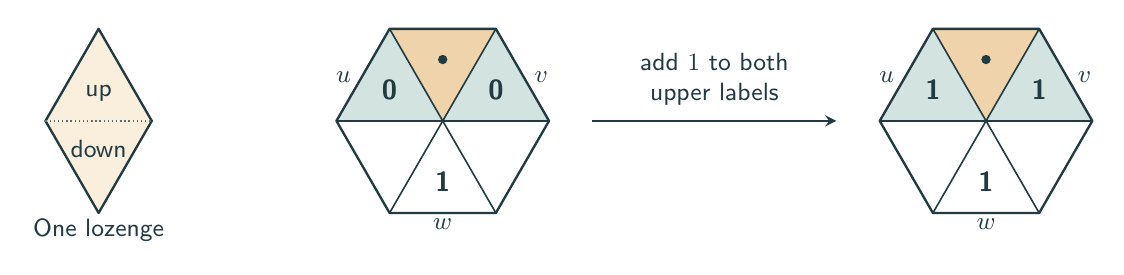
\begin{tikzpicture}[text=boxink,font=\sffamily\small,line join=round,>=stealth]
    \begin{scope}[shift={(-7.82,0)},scale=1.35]
      \filldraw[fill=boxtop!38,draw=boxink,line width=.85pt]
        (-.5,0)--(0,.8660254)--(.5,0)--(0,-.8660254)--cycle;
      \draw[draw=boxink!74,line width=.50pt,densely dotted] (-.5,0)--(.5,0);
      \node at (0,.26) {up};
      \node at (0,-.26) {down};
    \end{scope}
    \node[anchor=north,inner sep=2pt] at (-7.82,-1.17) {One lozenge};
    \foreach \offset/\upperentry in {-3.45/0,3.45/1}{%
      \begin{scope}[shift={(\offset,0)},scale=1.35]
        \fill[boxwarm!62] (0,0)--(60:1)--(120:1)--cycle;
        \fill[boxleft!42] (0,0)--(120:1)--(180:1)--cycle;
        \fill[boxleft!42] (0,0)--(0:1)--(60:1)--cycle;
        \foreach \angle in {0,60,...,300}
          \draw[boxink,line width=.58pt] (0,0)--(\angle:1);
        \draw[boxink,line width=.85pt]
          (0:1)--(60:1)--(120:1)--(180:1)--(240:1)--(300:1)--cycle;
        \fill[boxink] (0,.57735) circle[radius=1.25pt];
        \node[font=\sffamily\normalsize\bfseries] at (-.5,.288675) {\upperentry};
        \node[font=\sffamily\normalsize\bfseries] at ( .5,.288675) {\upperentry};
        \node[font=\sffamily\normalsize\bfseries] at (0,-.57735) {1};
        \node[anchor=east,inner sep=1.5pt] at (-.82,.41) {\(u\)};
        \node[anchor=west,inner sep=1.5pt] at ( .82,.41) {\(v\)};
        \node[anchor=north,inner sep=2pt] at (0,-.8660254) {\(w\)};
      \end{scope}}
    \draw[->,boxink,line width=.8pt] (-1.55,0)--(1.55,0);
    \node[above=2pt,align=center] at (0,0) {add \(1\) to both\\upper labels};
  \end{tikzpicture}}

\newcommand{\DegreeRow}[1]{%
  \draw[boxgrid,line width=.5pt] (0,#1)--(5,#1);
  \foreach \n in {0,1,4,5}{
    \node[draw=boxink,fill=boxleft!47,circle,inner sep=0pt,
          minimum size=12.5pt,line width=.5pt] at (\n,#1) {\n};}
  \foreach \n in {2,3}{
    \node[draw=boxgrid,fill=white,text=boxink!75,circle,inner sep=0pt,
          minimum size=12.5pt,line width=.45pt] at (\n,#1) {\n};}}
\newcommand{\ResiduePairs}{%
  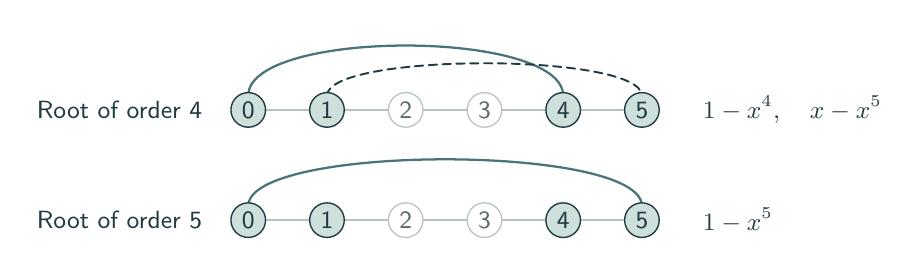
\begin{tikzpicture}[x=1.00cm,y=1cm,font=\sffamily\small,text=boxink,line cap=round]
    \node[anchor=east] at (-.46,1.35) {Root of order 4};
    \draw[boxright!80!black,line width=.82pt]
      (0,1.53) .. controls (0,2.38) and (4,2.38) .. (4,1.53);
    \draw[boxink,line width=.70pt,densely dashed]
      (1,1.53) .. controls (1,2.08) and (5,2.08) .. (5,1.53);
    \DegreeRow{1.35}
    \node[anchor=west] at (5.65,1.35) {\(\displaystyle 1-x^4,\quad x-x^5\)};
    \node[anchor=east] at (-.46,-.05) {Root of order 5};
    \draw[boxright!80!black,line width=.82pt]
      (0,.13) .. controls (0,.92) and (5,.92) .. (5,.13);
    \DegreeRow{-.05}
    \node[anchor=west] at (5.65,-.05) {\(\displaystyle 1-x^5\)};
  \end{tikzpicture}}

\usepackage[colorlinks=true,linkcolor=blue!40!black,citecolor=blue!40!black,
  urlcolor=blue!40!black]{hyperref}
\hypersetup{pdftitle={Boxes with cyclic tiling groups have one layer or size 2×2×4},
  pdfauthor={twinheterodox}}
\newtheorem{theorem}{Theorem}
\newtheorem{lemma}[theorem]{Lemma}
\newtheorem{corollary}[theorem]{Corollary}
\newcommand{\Z}{\mathbb Z}
\newcommand{\Q}{\mathbb Q}
\newcommand{\F}{\mathbb F}
\newcommand{\ord}{\operatorname{ord}}
\newcommand{\coker}{\operatorname{coker}}
\newcommand{\laur}{\Q[q,q^{-1}]}
\newcommand{\pos}[1]{(#1)_+}
\title{\Large\bfseries Boxes with cyclic tiling groups have one layer or size \(2\times2\times4\)}
\author{twinheterodox\\[2pt]\normalsize Prepared with Codex}
\date{19 November 2026}
\makeatletter
\renewcommand{\@maketitle}{%
  \begin{center}
    {\@title\par}\vspace{.6em}
    {\large\begin{tabular}{c}\@author\end{tabular}\par}\vspace{.45em}
    {\large\@date\par}
  \end{center}}
\makeatother
\begin{document}
\maketitle

\begin{abstract}
Kuperberg asked how a box's dimensions determine its tiling group.
We prove Conlon's conjecture that this group is cyclic exactly when one
side has length one or the box has dimensions \(2\times2\times4\) in some order.
For every box, we also show that the minimum number of generators of its
tiling group equals the largest multiplicity of a cyclotomic factor of
prime-power index in MacMahon's volume polynomial.
This polynomial counts stacks by the number of cubes they contain.
It also determines the Smith factors over \(\Q[q,q^{-1}]\) of the box's
weighted Carlitz matrix, which presents the tiling group at \(q=1\). Each
cyclotomic factor of multiplicity \(e\) occurs in exactly the last
\(e\) Smith factors, once in each.
\end{abstract}

\section{Which boxes have a cyclic tiling group?}

Stack unit cubes in a corner of an \(a\times b\times c\) box so that
column heights weakly decrease away from that corner in both horizontal
directions. This \emph{boxed plane partition} projects to a hexagon tiled
by diamonds called \emph{lozenges} (Figure~\ref{fig:stack}). The matrix
\(K\) of possible tile placements presents a finite abelian group
\(G(a,b,c)\), the \emph{tiling group}, with one generator for each row
and one relation for each column (Figure~\ref{fig:unit-placement}).
Its order is \(\lvert\det K\rvert\), the number of possible stacks
in that box~\cite[p.~265]{Propp}. In 1998 Kuperberg asked which group
of that order occurs for each box~\cite[Question~2]{Kuperberg1998}.

\begin{theorem}[Conlon's conjecture on cyclic tiling groups]\label{thm:cyclic}
For positive integers \(a,b,c\), the group \(G(a,b,c)\) is cyclic if
and only if some side has length one or \((a,b,c)\) is a permutation
of \((2,2,4)\). The exceptional group \(G(2,2,4)\) is isomorphic to
\(\Z/105\Z\).
\end{theorem}

Theorem~\ref{thm:cyclic} tells us when one generator suffices. How many
generators does an arbitrary box need? Give each stack of \(v\) cubes
weight \(q^v\) and sum over all stacks to obtain MacMahon's volume
polynomial \(M(q)\)~\cite[\S429]{MacMahon}. Write \(e(d)\) for the
multiplicity in \(M(q)\) of \(\Phi_d(q)\), the cyclotomic polynomial
whose roots are the primitive \(d\)th roots of unity.

\begin{theorem}[Minimum number of generators]\label{thm:generators}
The tiling group \(G(a,b,c)\) needs exactly \(\max_{p,j} e(p^j)\)
generators, where \(p\) runs over the primes and \(j\) over the positive integers.
\end{theorem}

\enlargethispage{1.1\baselineskip}
\begin{figure}[H]
\centering\StackAndTiling
\caption{One of the 105 stacks in the \(2\times2\times4\) box. Its
four columns have heights \(4,2,1,0\). Viewed along a body diagonal,
each visible unit square, whether the face
of a cube or part of the box's floor or walls, projects to a lozenge.
Together these lozenges tile the hexagon on the right, with the floor
and walls shown in pale colors. The dotted segment in the bottom
lozenge is its short diagonal. It determines that tile uniquely because
the two unit equilateral triangles with this common side form the lozenge.}
\label{fig:stack}
\end{figure}

Kuperberg observed that the tiling group of a one-layer box is
cyclic~\cite[Question~2]{Kuperberg1998}. In 2002 he proposed two
conjectures that together would determine the group for every
box~\cite[\S5.1, Conjectures~11--12]{Kuperberg}.
Conlon found the exceptional \(2\times2\times4\) box by computer and conjectured that it was the only
exceptional case~\cite[\S7]{Conlon}. MacMahon's count of the stacks~\cite[\S429]{MacMahon}
gives the group order \(105=3\cdot5\cdot7\), so by Cauchy's theorem there are
elements of orders \(3\), \(5\), and \(7\). Since these elements commute and
their orders are pairwise coprime, their product has order \(105\) and
generates the group.
Section~\ref{sec:cyclic-proof} rules out the remaining boxes by a gcd
calculation when the shortest side is two and by a bound on element
orders when it is larger.
Section~\ref{sec:volume} illustrates Theorem~\ref{thm:generators} on two
boxes with twenty stacks, and Section~\ref{sec:ordinary} proves it.

\subsection*{From the picture to the group}

The three orientations of a lozenge correspond to squares parallel to
the floor or to either wall. Projection gives a bijection
between stacks in an \(a\times b\times c\) box and lozenge tilings of
the equiangular hexagon with successive side lengths \(a,b,c,a,b,c\)%
~\cite[\S5.1, Fig.~10]{Kuperberg}.

Marking the short diagonal of every lozenge records the whole tiling.
To list the possible marks, divide the hexagon into unit triangles.
In the orientation of Figures~\ref{fig:stack} and~\ref{fig:unit-placement}, the right-pointing
triangles (\(\triangleright\)) index the rows of a matrix \(K\)
and the left-pointing ones (\(\triangleleft\)) its columns.
Put \(1\) for a shared side, the short diagonal of a possible tile,
and \(0\) otherwise. A choice gives a tiling exactly when its tiles
cover each triangle once, selecting one \(1\) per row and
column~\cite[p.~261]{Propp}. The Kasteleyn--Percus formula
counts these tilings by \(|\det K|\)~\cite[p.~265]{Propp}.

The generators of \(G(a,b,c)\) are indexed by the rows of \(K\). For
each column, set the sum of the generators at its \(1\)'s equal to
zero. In the one-cube box (Figure~\ref{fig:unit-placement}), column \(A\)
gives \(y=-x\), and then column \(B\) gives \(z=-y=x\). Substituting
in column \(C\) leaves one generator \(x\) with the single relation \(2x=0\).

With \(m\) triangles of each orientation, this construction gives the
quotient \(G=\Z^m/K\Z^m\), the integer cokernel of \(K\). Its order
is the lattice index \(|\det K|\). Kuperberg also asked how its elements
could be interpreted in terms of the tilings~\cite[p.~265, Problem~5]{Propp}.

\begin{figure}[!htbp]
\centering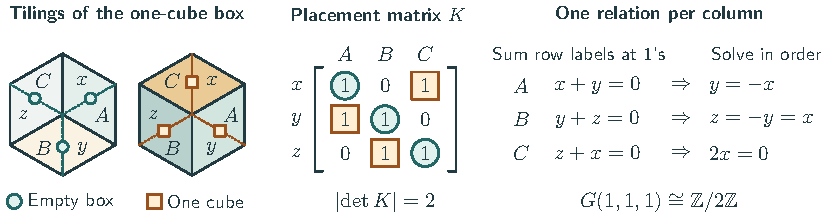
\includegraphics[width=\linewidth]{figures/one-cube-placement-matrix.pdf}
\caption{The marked diagonals of each tiling select one \(1\) in every
row and column of \(K\). Triangle \(A\) shares a lozenge with \(x\) in
the empty box and with \(y\) in the full box. In column \(A\) these two
lozenges give a circled \(1\) in row \(x\) and a boxed \(1\) in row
\(y\). Adding those row labels gives the group relation \(x+y=0\).}
\label{fig:unit-placement}
\end{figure}
\enlargethispage*{\baselineskip}

\subsection*{Does the stack count determine cyclicity?}

Both boxes in Figure~\ref{fig:twenty} have twenty stacks, and only the
flat box's tiling group is cyclic. Each colored line traces the boundary
of a layer halfway up its cubes, continuing along the box walls where
needed. Adding a unit cube interchanges two consecutive steps in its layer's path and
leaves its endpoints fixed. The \(\binom63=20\) shortest paths between
opposite floor corners give all the flat stacks. In the pictured
\(2\times2\times2\) box, three unit cubes form an L and a fourth sits
above its corner. Figure~\ref{fig:volumes} shows all twenty stacks in this box.

Kuperberg's path matrix presents the same group as the triangle matrix
\(K\)~\cite[Corollary~7 and Theorem~14]{Kuperberg}. Its rows index path starts
(generators) and its columns index path ends (relations). Each entry counts
paths between its endpoints by rising or falling steps to the right.
The flat box gives \(20x=0\). In the two-layer box, two of four steps rise
for a level finish (six choices), and one or three rise for a change of height
(four choices).

The upper path start gives \(x\) and the lower gives \(y\). In \(mx+ny\),
both relations preserve the parities of \(m,n\) because their coefficients
are even. All four pairs occur at \(0,x,y,x+y\). Multiples of any \(g\) give
only the parities of \(0\) or \(g\), so two generators are necessary.

\begin{figure}[!htbp]
\centering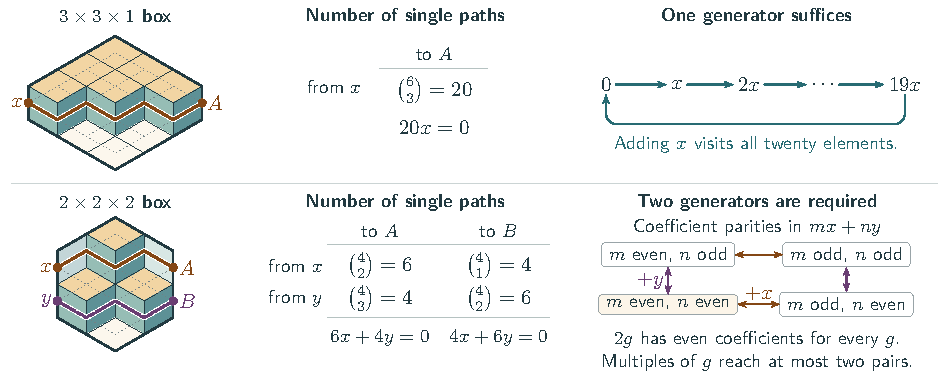
\includegraphics[width=\linewidth]{figures/equal-count-boxes.pdf}
\caption{Both boxes have twenty stacks. \(G(3,3,1)\) needs one generator
and \(G(2,2,2)\) needs two.
The colored paths trace the layers on the dotted grid. The lower right records
the coefficient parities in \(mx+ny\), so \(2x+y\) gives (even, odd).
Adding \(x\) changes only the parity of \(m\), and adding \(y\) only that of \(n\).}
\label{fig:twenty}
\end{figure}

\FloatBarrier
\section{What the volume polynomial remembers}\label{sec:volume}

A cyclic group contains an element of order \(|G|\). To rule this out
for every box with shortest side at least three, we bound the orders of
its elements using the volume polynomial. Figure~\ref{fig:volumes} sorts the twenty stacks in
the \(2\times2\times2\) box by volume. A rule that always adds or removes
one unit cube sends all twelve even-volume stacks into the eight odd-volume
stacks. Such a rule cannot realize addition by a group element, which is a
bijection.

\begin{figure}[htbp]
\centering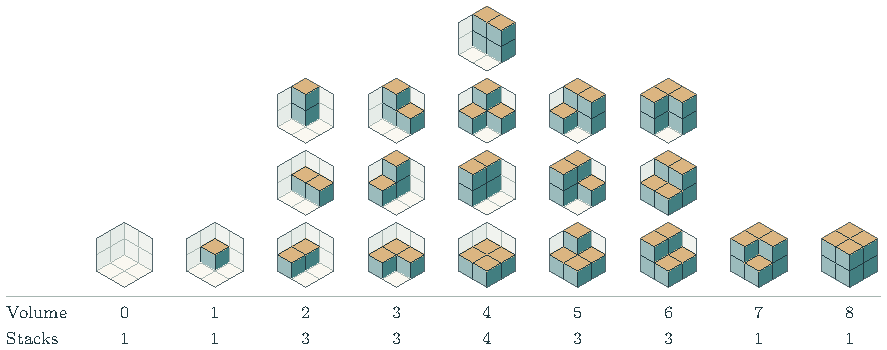
\includegraphics[width=.97\linewidth]{figures/volume-stacks.pdf}
\caption{The twenty stacks in the \(2\times2\times2\) box, arranged by
number of cubes. The darker faces belong to the cubes and the pale
faces belong to the box. Setting \(q=1\) counts all twenty stacks.}
\label{fig:volumes}
\end{figure}
\FloatBarrier

The four stacks in the middle column contribute \(4q^4\). Reading across
the figure gives the volume polynomial
\[
 M(q)=1+q+3q^2+3q^3+4q^4+3q^5+3q^6+q^7+q^8=A^2B,
\]
where \(A=1+q^2=\Phi_4(q)\) and \(B=1+q+q^2+q^3+q^4=\Phi_5(q)\).
The factor \(\Phi_4\) has prime-power index \(4=2^2\) and occurs twice,
so by Theorem~\ref{thm:generators} the group needs exactly two generators. For the flat
\(3\times3\times1\) box, MacMahon's product gives
\(M(q)=\Phi_2(q)\Phi_4(q)\Phi_5(q)\Phi_6(q)\). Each factor of
prime-power index occurs once, so one generator suffices. Both polynomials give
\(20\) at \(q=1\).

\Needspace{6\baselineskip}
The map \(mx+ny\mapsto(m\bmod2,(m+n)\bmod10)\) respects both relations
for the \(2\times2\times2\) box in Figure~\ref{fig:twenty} and takes all twenty values.
Since the group has order twenty, this gives
\(G(2,2,2)\cong\Z/2\Z\oplus\Z/10\Z\).
To see these summand orders in the volume polynomial, number the four
steps of each path in Figure~\ref{fig:twenty} from \(0\) to \(3\).
Give a rise weight \(1\) and a fall at position \(r\) weight \(q^r\),
and multiply the weights along the path. Choosing \(q^r u\) in
\(\prod_{r=0}^3(1+q^r u)\) records a fall at \(r\), so the coefficient
\(e_k\) of \(u^k\) counts paths with \(k\) falls by weight. From the
upper start \(x\) to the lower endpoint \(B\) there are three falls,
giving \(e_3\) in the upper-right entry. At \(q=1\) every path has weight one.
\[
 C(q)=\begin{pmatrix}e_2&e_3\\e_1&e_2\end{pmatrix},
 \qquad C(1)=\begin{pmatrix}6&4\\4&6\end{pmatrix}.
\]

The determinant of \(C(q)\) is \(M(q)\) times a power of \(q\).
Allow rational coefficients and powers of \(q\) of either sign. Invertible
row and column operations then give a diagonal matrix with each entry
dividing the next. These entries are the \emph{Smith factors}, determined
up to nonzero rational constants and powers of \(q\).

The first Smith factor divides the second, so its square divides \(A^2B\).
Since \(A\) and \(B\) are distinct irreducibles, the only possibilities
are \((1,A^2B)\) and \((A,AB)\). At \(q=i\), where
\(A=0\), the first has rank one and the second has rank zero.
The row and column operations remain invertible at \(i\), so we can
read the rank from \(C(i)\).

At this value the product defining the entries becomes
\((1+u)(1+iu)(1-u)(1-iu)=1-u^4\). All three middle coefficients
vanish, so \(C(i)=0\). This selects \((A,AB)\), giving the summand
orders \(2\) and \(10\) at \(q=1\).

\Needspace{7\baselineskip}
\subsection*{The rule for every box}

For the general box, fix the lengths \(a,b,c\), put \(N=b+c\), and
let \(e_k\) be the coefficient of \(x^k\) in
\(\prod_{j=0}^{N-1}(1+q^j x)\), with \(e_k=0\) outside \(0\le k\le N\).
The weighted Carlitz matrix and MacMahon's volume formula
\cite[\S429]{MacMahon} are
\[
 C=(e_{b-i+j})_{0\le i,j<a}, \qquad
 M(q)=\prod_{i=1}^{b}\prod_{j=1}^{c}
          \frac{1-q^{a+i+j-1}}{1-q^{i+j-1}}.
\]
Kuperberg relates \(C\), the dual Jacobi--Trudi matrix of the
rectangle \((a^b)\), to the weighted tiling matrix by invertible row
and column operations and adjoining identity blocks. He asks about
a diagonal form with squarefree entries over the integral Laurent
ring~\cite[Theorem~14 and Conjectures~11--12]{Kuperberg}. For ordinary
boxes we determine the factors over the rational Laurent ring.
If an irreducible factor occurs \(e\) times in the volume
polynomial, it goes in \(e\) different diagonal entries. Since each
entry divides the next, these must be the last \(e\).

\begin{theorem}\label{thm:smith}
Let \(\Phi_d\) denote the \(d\)-th cyclotomic polynomial and put
\(e(d)=\ord_{\Phi_d}M(q)\). In increasing divisibility order, the Smith
factors of \(C\) over \(\laur\), up to units, are
\[
             s_j(q)=\prod_{d:\,e(d)\ge a-j+1}\Phi_d(q),
             \qquad 1\le j\le a .
\]
\end{theorem}

For the \(2\times2\times2\) box, \(A=\Phi_4\) occurs twice and \(B=\Phi_5\) occurs
once. For arbitrary boxes, the operations used over the rational
Laurent ring can introduce integer denominators. To draw conclusions
about the tiling group at \(q=1\), Section~\ref{sec:integer}
therefore proves divisibility for the determinants of square
submatrices before setting \(q=1\).

The rank test at \(q=i\) suggests how to prove the weighted theorem.
At a primitive \(d\)-th root of unity the determinant vanishes to
order \(e(d)\). Each diagonal entry that vanishes uses at least one
of those \(e(d)\) factors and lowers the rank by one. We will find
\(e(d)\) independent vectors sent to zero, forcing all \(e(d)\)
copies into different entries.

\section{The two intervals of exponents}

Write the \(a\) coordinates of a vector as the coefficients of a
polynomial \(f(x)\) of degree \(<a\). Put
\(g(x)=\prod_{j=0}^{N-1}(1-q^j x)\). Multiplying \(f\) by \(g\)
and taking the coefficients of
\(x^b,\ldots,x^{b+a-1}\) gives \(C^{\mathsf T}\) up to row and column
signs. Indeed, coefficient \(i\) in this block applied to \(x^j\) is
\((-1)^{b+i-j}e_{b+i-j}\). The coefficient map sends a vector to zero
precisely when these middle coefficients vanish. Its product \(gf\)
can then have nonzero terms only in the two outside intervals.
Transposition and the signs preserve rank. Thus at any nonzero
specialization of \(q\) to a field, the nullity of \(C\) is the
dimension of the polynomials supported on
\begin{equation}\label{eq:E}
 E=\{0,\ldots,b-1\}\ \cup\ \{a+b,\ldots,a+b+c-1\}
\end{equation}
that are divisible by \(g\). Division recovers \(f\), since \(g\) has
degree \(N\) and \(\max E=a+N-1\).

\Needspace{13\baselineskip}
For the \(2\times2\times2\) box the allowed exponents are \(0,1,4,5\).
At \(q=i\) we have \(g(x)=1-x^4\), so both \(1-x^4\) and \(x-x^5\)
have the prescribed zeros and allowed support. They are independent.
At a primitive fifth root, \(g\) divides \(1-x^5\), which again has
allowed support. These give the two missing ranks at a fourth root and
the one missing rank at a fifth root, exactly the multiplicities we saw
in the volume polynomial. Figure~\ref{fig:degrees} shows how to find
the multiples before doing any division.

\begin{figure}[htbp]
\centering\ResiduePairs
\caption{A line joins two allowed powers whose exponents agree modulo
the order of the root. Their differences on the right are the supported
products \(P(x)=g(x)f(x)\). At the pale positions the coefficients
of \(P\) must vanish.}
\label{fig:degrees}
\end{figure}

The same support gives a short determinant calculation. Put
\(L=\{0,\ldots,N-1\}\). Use as columns the monomials \(x^k\), \(k\in E\)
in increasing order, followed by \(g,xg,\ldots,x^{a-1}g\), in the
monomial basis through degree \(a+N-1\). Expanding along the monomial
columns gives \((-1)^{aN}\det C\). Alternatively, use as coordinate basis
the monomials from \(L\) followed by the same multiples of \(g\).
The change of basis has determinant
\((-1)^{aN}q^{a\binom N2}\). In these coordinates the only determinant
left is that of the remainders of \(x^k\), \(k\in E\), modulo \(g\).
Over \(\Q(q)\), evaluation at \(q^{-i}\), \(0\le i<N\), computes this
last determinant as a quotient of Vandermonde determinants, one on
\((q^{-k})_{k\in E}\) and the other on \((q^{-k})_{k\in L}\).
Pairs within each interval cancel. The cross pairs give \(M(q)\), and
the powers of \(q\) give
\begin{equation}\label{eq:det}
             \det C=q^{a\binom b2}M(q).
\end{equation}
Indeed the cross differences in the numerator and denominator have
lengths \(a+b+j-i\) and \(b+j-i\) for \(0\le i<b\), \(0\le j<c\).
Shifting the last \(c\) exponents of \(L\) by \(a\) contributes the
monomial \(q^{-a\sum_{j=b}^{N-1}j}\) to the Vandermonde quotient.

Fix \(d\ge1\), write \(N=md+v\), \(0\le v<d\), and let \(n_r\) be the
number of elements of \(E\) congruent to \(r\bmod d\). Every difference
of distinct exponents contributes one factor \(\Phi_d\) precisely when
its two exponents agree modulo \(d\). Among the exponents in \(L\),
\(v\) residue classes have size \(m+1\) and the others have size \(m\).
Hence
\begin{equation}\label{eq:valuation}
 e(d)=\sum_{r=0}^{d-1}\binom{n_r}{2}
          -d\binom m2-mv
     =\sum_{r=0}^{d-1}\binom{n_r-m}{2}.
\end{equation}
The second identity uses \(\sum_r(n_r-m)=v\) and the polynomial
convention \(\binom{x}{2}=x(x-1)/2\), also at \(x=-1\).

\section{Finding all the missing ranks}

Let \(\zeta\) be a primitive \(d\)-th root of unity. At \(q=\zeta\)
one full period of factors in \(g\) gives \(1-x^d\). Thus
\[
      g(x)=(1-x^d)^m H(x),\qquad
      H(x)=\prod_{j=0}^{v-1}(1-\zeta^j x),\qquad H\mid 1-x^d .
\]
This gives two ways to construct a multiple of \(g\) with support in
\(E\). We can impose \(m+1\) full periods of zeros, or impose \(m\)
full periods and then the \(v\) remaining zeros.

The two rows of Figure~\ref{fig:degrees} show why we use both constructions.
At \(d=4\), one full period gives the two multiples \(1-x^4\) and
\(x(1-x^4)\). A second full period would require the factor
\((1-x^4)^2\), whose degree \(8\) exceeds the largest allowed exponent \(5\).
At \(d=5\), counting four
root conditions on four coefficients gives only the lower bound zero.
Completing the period gives the supported multiple \(1-x^5\).

\begin{lemma}\label{lem:null}
With \(t_+=\max(t,0)\), the nullity at \(q=\zeta\) is at least
\[
 \max\left\{\sum_r\pos{n_r-m-1},\
                      \sum_r\pos{n_r-m}-v\right\}.
\]
\end{lemma}
\begin{proof}
Write a supported polynomial uniquely as
\(P(x)=\sum_{r=0}^{d-1}x^r f_r(x^d)\). The coefficients of \(f_r\)
have \(n_r\) degrees of freedom. Requiring \((u-1)^h\mid f_r(u)\)
imposes at most \(h\) linear conditions, namely zero remainder modulo
\((u-1)^h\). The resulting space has dimension at least
\(\sum_r(n_r-h)_+\), and every \(P\) in it is divisible by
\((1-x^d)^h\). Choosing \(h=m+1\) gives the first bound. Choosing
\(h=m\), divide by \((1-x^d)^m\) and require zero remainder modulo \(H\).
This imposes at most \(v\) further conditions and gives the second bound.
\end{proof}

The shape of the box now enters. Each of the two intervals in
\eqref{eq:E} contributes either the floor or the ceiling of its length
divided by \(d\) to \(n_r\). Write \(b=Bd+\beta\), \(c=Dd+\gamma\),
with \(0\le\beta,\gamma<d\).

If \(\beta+\gamma<d\), then \(m=B+D\) and every \(n_r-m\) is
0, 1, or 2. In \eqref{eq:valuation} only the 2's contribute. Their number
is exactly the first lower bound in Lemma~\ref{lem:null}.

If \(\beta+\gamma\ge d\), then \(m=B+D+1\) and every \(n_r-m\)
is \(-1\), 0, or 1. Only the \(-1\)'s contribute to
\eqref{eq:valuation}. Their number is
\(\sum_r(n_r-m)_+-v\), since \(\sum_r(n_r-m)=v\).
This is the second lower bound. These arguments also cover \(d>N\)
and \(v=0\).

We have found at least \(e(d)\) dimensions of kernel. In Smith form
the nullity at \(\zeta\) counts the invariant factors divisible by
\(\Phi_d\). Their valuations sum to \(e(d)\) by \eqref{eq:det}, so there
are exactly \(e(d)\) of them, each of valuation one. Divisibility puts
them in the last \(e(d)\) positions. All nonunit irreducibles of the
determinant are cyclotomic, which proves Theorem~\ref{thm:smith}.

There are exactly \(\min(a,b,c)\) nonunit rational Laurent factors. For
\(a\le b\le c\), at a primitive \((b+c)\)-th root the product defining
the elementary functions has only its constant and top coefficients,
and every matrix entry is intermediate. Thus the entire matrix vanishes.
Permuting the box sides preserves \(M\), so the number \(\max_d e(d)\)
has the same value in every orientation. This also gives the count
proposed in \cite[\S9]{Conlon} for an integral Laurent Smith form
if it exists, since primitivity of the determinant precludes
additional nonunit constant factors.

\section{Consequences for the integer matrix}\label{sec:integer}

Let \(G=\coker C(1)\), the quotient of \(\Z^a\) by the image of the
integer Carlitz matrix. Its order is \(M(1)\). For \(0\le k\le a\) put
\[
       D_k(q)=\prod_{d\ge2}\Phi_d(q)^{(e(d)-a+k)_+}.
\]
Over \(\laur\) the product of the first \(k\) Smith factors divides every
\(k\)-rowed minor. That product is \(D_k(q)\). Its coprimality to \(q\)
lets us remove powers of \(q\) over \(\Q[q]\). Division by the monic
polynomial \(D_k(q)\) then proves divisibility of the actual minors
in \(\Z[q]\). This makes specialization legitimate
even if rational row operations would introduce denominators.

\begin{corollary}\label{cor:int}
Every \(k\)-rowed minor of \(C(1)\) is divisible by \(D_k(1)\). In
particular, the exponent of \(G\) divides
\[
      \prod_{\substack{d\ge2\\e(d)>0}}\Phi_d(1)
      \quad\text{which divides}\quad
      \operatorname{lcm}(1,\ldots,a+b+c-1).
\]
\end{corollary}
\begin{proof}
The exponent of \(G\), the largest order of one of its elements, is
its last integer Smith factor. This is \(M(1)\) divided by the gcd of
the cofactors, with gcd 1 in size one. For the \(2\times2\times2\) box
the diagonal cofactors are \(6\) and the off-diagonal cofactors are
\(-4\). Their gcd is \(2\), so the
largest element order is \(20/2=10\). In general \(D_{a-1}(1)\)
divides the cofactor gcd. Dividing \(M(1)\) by \(D_{a-1}(1)\) gives
the stated product. All indices \(d\) occurring are at most
\(\max E=a+b+c-1\). For \(d\ge2\), \(\Phi_d(1)=p\) if \(d\) is
a positive power of a prime \(p\), and is 1 otherwise. This gives both
the lcm bound and \(\ord_p |G|=\sum_{j\ge1}e(p^j)\).
\end{proof}

\section{Proof of the cyclicity classification}\label{sec:cyclic-proof}

\begin{proof}[Proof of Theorem~\ref{thm:cyclic}]
Order the sides \(a\le b\le c\). Permuting them gives stably equivalent
presentations of the same tiling group~\cite[Problem~5]{Propp}.
If \(a=1\), the Carlitz matrix has a single entry and the group is cyclic.

If \(a=2\), the group is cyclic exactly when the entries of the
two-by-two Carlitz matrix have gcd \(1\), since their gcd is its first
Smith factor. Put \(U=\binom{b+c}{b}\). The diagonal entries are \(U\),
and the other two are \(Ub/(c+1)\) and \(Uc/(b+1)\). Their gcd is at least
\(U/((b+1)(c+1))\), because multiplication by \((b+1)(c+1)\) makes
all three entries integer multiples of \(U\). The lower bound increases
with either \(b\) or \(c\) for \(b,c\ge2\) and equals \(20/16\) at \(b=c=3\).
For \(b=2\) it is \((c+2)/6>1\) whenever \(c\ge5\).
Finally at \(b=2,\ c=2,3,4\) the gcds are respectively \(2,5,1\).
Only the last box gives a cyclic group. Its matrix
\(\left(\begin{smallmatrix}15&20\\6&15\end{smallmatrix}\right)\)
has determinant \(105\). The map \((x,y)\mapsto5y-9x\bmod105\)
sends both columns to zero and the class of \((1,2)\) to \(1\), giving
an explicit isomorphism with \(\Z/105\Z\).

Suppose now that \(a\ge3\). A finite abelian group is cyclic exactly
when its exponent equals its order. We show that the order outgrows an
upper bound for the exponent.

Write \(t=a+b-1\) and \(L(t)=\operatorname{lcm}(1,\ldots,t)\).
Each active power \(p^j\) divides a numerator index in the symmetric
version of MacMahon's formula having height \(c\). These indices range
from \(c+1\) to \(c+t\). The number of active levels is at most the
largest active \(j\), so Corollary~\ref{cor:int} gives
\[
 \exp(G)\mid\operatorname{lcm}(c+1,\ldots,c+t)
             \mid L(t)\binom{c+t}{t}.
\]
For the second divisibility, every power of a prime beyond \(t\) that
divides some \(c+i\) contributes to the valuation of the binomial,
and the smaller powers are covered by \(L(t)\).
In the product for \(|G|\), the cells of the first row and last column
together give one factor \(1+c/k\) for every \(1\le k\le t\). Thus
\[
 F(a,b,c)=\frac{|G|}{\binom{c+t}{t}}
       =\prod_{i=2}^{a}\prod_{j=1}^{b-1}\left(1+\frac{c}{i+j-1}\right).
\]
It suffices that \(F(a,b,c)>L(t)\), and \(F\) increases with \(c\).

For \(b\ge7\) it suffices to compare \(F(a,b,b)\) with the upper bound
\(4^{t-1}\) for \(L(t)\). Start at \((3,7,7)\), increase \(b\) along
\((3,b,b)\), and then increase \(a\) at fixed \(b\). Each step adds
one to \(t=a+b-1\), multiplying the comparison bound by four.

To prove \(L(n)\le4^{n-1}\) by induction, observe that
\(L(2m)/L(m)\) divides \(\binom{2m}{m}\), and
\(L(2m+1)/L(m+1)\) divides \(\binom{2m+1}{m}\). Any prime power
missing from the smaller lcm gives a factor in the binomial, and at most
one power per prime is missing. Both binomials are at most \(4^m\), using
the two equal central coefficients in the odd row.
For \(F_b=F(3,b,b)\), multiplying its two rows gives
\[
 F_b=\frac{2(2b+1)\binom{2b}{b}^2}{(b+1)^3(b+2)},\qquad
 \frac{F_{b+1}}{F_b}=
 \frac{4(2b+3)(2b+1)(b+1)}{(b+2)^2(b+3)}>4 \quad(b\ge2).
\]
The last inequality reduces to \(3b^3+5b^2-5b-9>0\).
Since \(F_7=306735/4>4^8\), we have \(F_b>4^{b+1}\).
Each new row up to \(a\le b\) increases \(F(a,b,b)\) by a factor of
at least \((3/2)^{b-1}>4\). Therefore \(F(a,b,c)>4^{a+b-2}\ge L(t)\).

For \(4\le b\le6\) the first pair of columns below covers \(a=3\).
The second covers every \(4\le a\le b\), by monotonicity of \(F\) and
\(L(t)\le L(2b-1)\).
\[
\begin{array}{c|rr|rr}
 b &F(3,b,b)&L(b+2)&F(4,b,b)&L(2b-1)\\ \hline
 4&588/5&60&3528/5&420\\
 5&924&420&13068&2520\\
 6&56628/7&840&2024451/7&27720
\end{array}
\]
For \(a=b=3\) and \(c\ge6\), \(F(3,3,6)=90>60=L(5)\).
For \(c=3,4,5\) the respective group orders are \(980,4116,14112\),
while \(\operatorname{lcm}(c+1,\ldots,c+5)\) is \(840,2520,2520\).
This proves noncyclicity for every box with minimum side at least three
and completes the classification.
\end{proof}

Another prediction in Conlon's \S7 concerns the number of generators
for an \(n\times n\times n\) box. It requires \(n\) generators exactly
when \(n\) is a power of two, including \(n=1\). Indeed this happens
when some prime divides every entry. The entries comprise all interior
binomial coefficients of row \(2n\). If \(2n=p^h u\), \(p\nmid u\),
then \((1+X)^{2n}=(1+X^{p^h})^u\) in \(\F_p[X]\). All interior
coefficients vanish when \(u=1\), while for \(u>1\) the coefficient at
\(p^h\) is \(u\ne0\). Hence \(2n\) must be a prime power, and the prime must be 2.

\section{The ordinary group at a prime}\label{sec:ordinary}

The four coefficient-parity pairs in Figure~\ref{fig:twenty} form
\(G/2G\) for the \(2\times2\times2\) box. Both relations vanish modulo
\(2\), leaving the images of \(x,y\) as a basis over \(\F_2\).
For any box and prime \(p\), reducing the generators and relations modulo \(p\) gives
\(G/pG\), with one dimension for each nontrivial cyclic summand of
the \(p\)-primary subgroup \(G_p\).

Call \(j\ge1\) active if \(e(p^j)>0\), and let \(t_p\) count the active
indices. Corollary~\ref{cor:int} gives \(\lvert G_p\rvert\) and
\(p^{t_p}G_p=0\). Since \(C(1)\) is square, its nullity modulo \(p\)
equals \(\dim_{\F_p}(G/pG)\). We compute it using Han's theorem on
relations between three powers of linear forms.

\begin{theorem}\label{thm:ordinary}
For every \(p\) the dimension of \(G/pG\) over \(\F_p\) is
\(\max_{j\ge1} e(p^j)\), with empty maximum zero. If \(t_p\le2\),
list the positive multiplicities \(e(p^j)\) and pad the list with zeros
to obtain two numbers \(u\le v\). Then
\[
          G_p \ \simeq\ (\Z/p)^{\,v-u}\oplus(\Z/p^2)^{\,u}.
\]
This gives the complete \(p\)-primary group for every
\(p^3>a+b+c-1\), and also for smaller primes having at most two active
indices.
\end{theorem}

\begin{proof}[Deduction of Theorem~\ref{thm:generators}]
Write \(G\) as a direct sum of cyclic groups of orders \(1<n_1\mid\cdots\mid n_r\).
One generator from each summand suffices. Any generating set of \(G\)
maps to a spanning set of \(G/pG\). A prime \(p\) dividing \(n_1\) divides
every \(n_i\), giving \(G/pG\cong\F_p^r\). The minimum for \(G\) is
therefore \(\max_p\dim_{\F_p}(G/pG)=\max_{p,j} e(p^j)\) by
Theorem~\ref{thm:ordinary}.
\end{proof}

To prove Theorem~\ref{thm:ordinary}, we first express \(e(d)\) in
terms of the side lengths modulo \(d\). Let
\(x,y,z\) be the least nonnegative residues of \(a,b,c\bmod d\) and
\(S=x+y+z\). For \(d\ge2\),
\begin{equation}\label{eq:tent}
 e(d)=\max\{0,\min(x,y,z,d-x,d-y,d-z,S-d,2d-S)\}.
\end{equation}
Indeed, with \(F(h)=\sum_{i=0}^{h-1}\lfloor i/d\rfloor\), the
factorial form of the product in \eqref{eq:det} gives
\[
 F(a+b+c)+F(a)+F(b)+F(c)-F(a+b)-F(a+c)-F(b+c).
\]
The identity \(F(h+d)=F(h)+h\) permits reduction of each side length
modulo \(d\). Since \(F(h)=\sum_{l\ge1}(h-ld)_+\), the expression becomes
\[
 (S-d)_++(S-2d)_+-(x+y-d)_+-(x+z-d)_+-(y+z-d)_+.
\]
It vanishes for \(S\le d\) and \(S\ge2d\). In the remaining range order
\(x\le y\le z\) and put \(w=S-d\). The expression is
\(w-(w-x)_+-(w-y)_+-(w-z)_+\). As \(w\) crosses \(x,y,z\), this takes
the successive forms \(w,x,d-z,2d-S\), giving \eqref{eq:tent}.

For example, take a cubical box of side \(2^h+1\) with \(h\ge2\). In
\eqref{eq:tent} the only active powers of 2 are \(2\) and \(2^{h+1}\),
with multiplicities 1 and \(2^h-3\). At the intermediate powers
all three residues are 1 and their sum is less than \(d\). At higher
powers even the original three sides sum to less than \(d\).
Theorem~\ref{thm:ordinary} thus gives
\[
        G_2\simeq(\Z/2)^{\,2^h-4}\oplus\Z/4 .
\]
In particular the \(9\times9\times9\) box has four summands of order 2
and one of order 4.

\begin{proof}[Proof of Theorem~\ref{thm:ordinary}]
Put \(T=a+b+c\), \(A=a+b\), \(B=a+c\), \(W=b+c\), and work over the
algebraic closure \(k\) of \(\F_p\), which preserves the nullity.
In \(k[X,Y]/(X^A,Y^B)\), multiply by \((X+Y)^W\) from degree \(a-1\)
to degree \(T-1\). The source monomials have \(X\)-exponents
\(0,\ldots,a-1\) and the target monomials have \(X\)-exponents
\(b,\ldots,b+a-1\). Thus the matrix is \(C(1)^{\mathsf T}\).
This use of multiplication in characteristic \(p\) is related to the
weak Lefschetz interpretation of prime divisibility of the box count in
Li and Zanello~\cite[Theorem~4.2]{LZ}.

Let \(\alpha\le\beta\) be the degrees of a homogeneous free basis for the
relations between \(X^A,Y^B,(X+Y)^W\) in \(k[X,Y]\). The relation module
is free of rank two by the graded syzygy theorem in two variables.
Its degrees satisfy \(\alpha+\beta=2T\) because the Hilbert-series numerator
\(1-t^A-t^B-t^W+t^\alpha+t^\beta\) of the finite-dimensional quotient
has a double zero at \(t=1\). The third coefficient of a relation of
degree \(T-1\) runs through precisely the kernel of our map. That
coefficient determines the whole relation, since the least degree of a
relation on \(X^A,Y^B\) alone is \(A+B>T-1\). It follows that
\[
      \dim_k\ker C(1)=(T-\alpha)_++(T-\beta)_+
                       =(\beta-\alpha)/2 .
\]

Han's theorem computes this degree gap by a distance. We use the
statement in Brenner and Kaid~\cite[Theorem~2.3]{BK}, which attributes
the formula to Han~\cite{Han} and also gives Monsky's proof
reference~\cite[Corollary~23]{Monsky}. Put \(\mathbf v=(W,B,A)\)
and let \(\mathcal O\) be the triples of integers with odd sum. Write
\(\operatorname{dist}_1\) for the sum-of-absolute-values distance to a
set. The coordinates of \(\mathbf v\) satisfy the strict triangle
inequalities. If \(s\) is the least integer for which
\(\operatorname{dist}_1(p^s\mathbf v,\mathcal O)<1\), the gap is
\[
 \beta-\alpha=p^{-s}\bigl(1-\operatorname{dist}_1(p^s\mathbf v,\mathcal O)\bigr).
\]
It is zero when there is no such \(s\). Coordinate permutations preserve
the formula. The sum of the coordinates of \(\mathbf v\) is even, so
only \(s<0\) can qualify.

For any \(d\ge2\) we claim that
\[
        \bigl(d-\operatorname{dist}_1(\mathbf v,d\mathcal O)\bigr)_+
                       =2e(d).
\]
Reducing the sides modulo \(d\) changes \(\mathbf v/d\) by an integer
triple with even sum. We can therefore use
\(\mathbf v'=(y+z,x+z,x+y)\). If an odd center \(d\mathbf h\) lies at
distance \(<d\), each of \(2x,2y,2z\) must be within \(d\) of an odd
multiple of \(d\). Indeed each is the sum of two coordinates of
\(\mathbf v'\) minus the third. In \([0,2d)\) the required odd multiple
can only be \(d\). The three equations on \(\mathbf h\) force
\(\mathbf h=(1,1,1)\). To compute the distance to this center, take
the largest absolute signed coordinate sum, allowing all signs.
Up to a common sign the four sums are
\(2x-d,2y-d,2z-d,2S-3d\). Taking the positive part of \(d\) minus their
maximum absolute value gives twice the minimum in \eqref{eq:tent}
when positive, and zero otherwise.

Han's least \(s\) therefore chooses the largest active power \(D=p^{-s}\).
It also gives the largest \(e(d)\) among the active powers. In fact, if
\(d,D=ld\) are both active and \(l>1\), take their closest odd centers
\(d\mathbf h,D\mathbf H\). The triangle inequality gives
\(\|\mathbf h-l\mathbf H\|_1<l+1\). This integer has parity \(1-l\),
so it is at most \(l-1\). Hence
\[
       D-\|\mathbf v-D\mathbf H\|_1
          \ \ge\ d-\|\mathbf v-d\mathbf h\|_1 .
\]
This proves the rank formula, also when no level is active. If at most
two levels occur, the \(v\) nontrivial cyclic \(p\)-power factors have
orders \(p\) or \(p^2\), and the base-\(p\) logarithm of the group order
is \(u+v\). Thus exactly \(u\) of those factors have order \(p^2\).
\end{proof}

\section{The first determinantal ideal over the integers}

For the entries themselves one can strengthen the divisibility in
Corollary~\ref{cor:int} to an equality of ideals before specializing.
The reason is that their indices run through a consecutive interval.
Write \(B_k(q)=\left[\begin{smallmatrix}N\\k\end{smallmatrix}\right]_q\)
for the Gaussian binomial coefficient. Up to a power of \(q\), \(e_k=B_k\)
for \(0\le k\le N\). Ekedahl's full-interior-row result, published by
Mirmohades~\cite[Theorem~3.1]{Mirmohades}, gives the ideal
\((\Phi_N)\) when the indices are \(1,\ldots,N-1\), \(N\ge2\).
Hazi's proof of Theorem~3.8 treats initial intervals in the two-colored
setting~\cite{Hazi}. Joris, Oestreicher and Steinig studied the gcd of
consecutive ordinary binomial coefficients~\cite{JOS}. Here we use any
nonempty consecutive interval \(I\subseteq\{0,\ldots,N\}\) in the
polynomial ring.

\begin{lemma}\label{lem:interval}
The \(B_k(q)\) for \(k\in I\) generate their monic polynomial gcd as an
ideal in \(\Z[q]\).
\end{lemma}
\begin{proof}
Let \(g_I\) be their monic gcd in \(\Q[q]\). The factorial formula
for Gaussian binomials gives
\[
 \ord_{\Phi_d} B_k
 =\left\lfloor\frac Nd\right\rfloor-\left\lfloor\frac kd\right\rfloor
  -\left\lfloor\frac{N-k}d\right\rfloor
 =\begin{cases}0,&k\bmod d\le N\bmod d,\\1,&k\bmod d>N\bmod d.\end{cases}
\]
Here \(d\ge2\), and these are all the irreducible factors. The quotients
\(B_k/g_I\) therefore belong to \(\Z[q]\) and have constant term 1.
Suppose their ideal were proper. A rational polynomial B\'ezout identity
gives a nonzero integer in that ideal after denominators are cleared,
so a maximal ideal containing it has residue characteristic \(p>0\).
Its residue field is a finite extension of \(\F_p\). The constant terms
force the image of \(q\) to be nonzero. Denote its multiplicative order by
\(n\). The cyclotomics vanishing there have indices \(d=np^j\), \(j\ge0\),
with \(d=1\) omitted from consideration. This follows from
\(X^{mp}-1=(X^m-1)^p\) in characteristic \(p\) and the distinct roots
of \(X^n-1\) when \(p\nmid n\).

For each such \(d\), call an index good if \(k\bmod d\le N\bmod d\).
If goodness is constant on \(I\) for every \(d\), any \(k\in I\) attains
all the minimum valuations. Otherwise take the largest \(D\) on this
chain for which there are both good and bad indices. Such \(D\) exists
because all indices are good for \(d>N\). The good indices modulo \(D\)
occur in the consecutive blocks
\([tD,tD+(N\bmod D)]\). Since \(I\) contains both kinds of index, it
contains a good endpoint of one of these blocks. That endpoint is
congruent to either \(0\) or \(N\) modulo \emph{every} divisor of \(D\),
so it is good for every smaller \(d\) on the chain. At every larger
level the choice of index is immaterial. Thus a single \(B_k\) attains
the minimum at every vanishing cyclotomic. Its quotient by \(g_I\)
is nonzero in the residue field, a contradiction.
\end{proof}

For \(C\) take \(I=[b-a+1,b+a-1]\cap[0,N]\) in the integers. Powers of
\(q\) are units in \(\Z[q,q^{-1}]\), so the entries generate
\((s_1(q))\) over the integral Laurent ring. In particular the smallest
ordinary Smith factor always equals \(s_1(1)\). The
two-by-two weighted presentation also has a Smith form in each local
ring at a maximal ideal, since after division by \(s_1\) one entry
is a unit and serves as a pivot.

\paragraph{Relation to earlier work.}
Kuperberg's integral Laurent problem also asks that the diagonal form
exist over \(\Z[q,q^{-1}]\). Theorem~\ref{thm:smith} determines it
after rational coefficients are allowed. In Stanley's Theorem~3.1
the alphabet length varies through \(y=q^N\), with \(y\)
independent and \(q\) in the coefficient field
\(\Q(q)\)~\cite{Stanley}. Here \(N\) is a fixed integer and the zeros
in the variable \(q\) determine the invariant factors. Chen, Guo, Jin
and Liu studied the integer Carlitz matrices and used skew Schur
polynomials to relate minors of Toeplitz matrices~\cite{CGJL}.
Huang and Yang's path formula and interval decompositions
\cite[\S\S4.2, 4.4]{HY} give a representation-theoretic method for
computing ranks at a fixed root of unity.
The length-\(N\) path between grades \(a-1\)
and \(a+N-1\) on the tensor product with interval lengths \(a+b-1\) and
\(a+c-1\) gives our transposed matrix up to row and column units.
For \(k=b+i-j\), the exponent adjustment from their
\(q^{j(N-k)}B_k(q)\) to \(e_k\) is
\(\binom{b+i}{2}-\binom j2-Nj\).

\paragraph{Kuperberg's question.}
In each cyclic case of Theorem~\ref{thm:cyclic}, the group is
\(\Z/M(1)\Z\). Choosing a side of length two for \(a\) gives a two-row
presentation. Lemma~\ref{lem:interval} gives the first integer Smith factor
\(s_1(1)\), and the determinant gives the second, \(M(1)/s_1(1)\).
For any box, Theorem~\ref{thm:ordinary} determines the entire
\(p\)-primary group whenever at most two of the polynomials
\(\Phi_{p^j}\), \(j\ge1\), divide \(M(q)\). With three or more such
indices, we still know the number of cyclic \(p\)-power summands.
Corollary~\ref{cor:int} supplies a common divisor of the minors of
\(C(1)\) at each intermediate size \(1<k<a\). The exact power of \(p\)
in the gcd at each size would determine the orders of the individual summands.

\section*{Verification}
Another AI model independently audited the mathematics and exposition of the
19 November 2026 draft. It found no gap in the proofs and used its own code
to compute the integer Smith forms for all 364 boxes with
\(1\le a\le b\le c\le12\).

\Needspace{11\baselineskip}
\begingroup
\small
\raggedright
\begin{thebibliography}{99}
\bibitem{BK} H. Brenner and A. Kaid, \emph{A note on the weak Lefschetz
property of monomial complete intersections in positive characteristic}.
\href{https://arxiv.org/abs/1003.0824}{arXiv:1003.0824}.
\bibitem{CGJL} C. Chen, A. Guo, X. Jin and G. Liu,
\emph{Trivariate monomial complete intersections and plane partitions},
\href{https://arxiv.org/abs/1008.1426}{arXiv:1008.1426}.
\bibitem{Conlon} N. Conlon, \emph{On plane partitions and Kasteleyn
cokernels}, UC Davis REU report, January 2022.
\href{https://web.archive.org/web/20220629185444id_/https://reu.math.ucdavis.edu/application/files/8416/5146/0704/conlon-report.pdf}{Archived report}.
\bibitem{Han} C. Han, \emph{The Hilbert--Kunz function of a diagonal
hypersurface}, Ph.D. thesis, Brandeis University, 1991.
\bibitem{Hazi} A. Hazi, \emph{Existence and rotatability of the
two-colored Jones--Wenzl projector}.
\href{https://doi.org/10.1112/blms.12983}{doi:10.1112/blms.12983}.
\bibitem{HY} H.-L. Huang and Y. Yang, \emph{The Green rings of minimal
Hopf quivers}. \href{https://doi.org/10.1017/S0013091515000085}{doi:10.1017/S0013091515000085}.
\bibitem{JOS} H. Joris, C. Oestreicher and J. Steinig,
\emph{The greatest common divisor of certain sets of binomial coefficients},
J. Number Theory \textbf{21} (1985), 101--119.
\href{https://doi.org/10.1016/0022-314X(85)90013-7}{doi:10.1016/0022-314X(85)90013-7}.
\bibitem{Kuperberg1998} G. Kuperberg, \emph{An exploration of the
permanent-determinant method}, Electron. J. Combin. \textbf{5} (1998), R46.
\href{https://doi.org/10.37236/1384}{doi:10.37236/1384}.
\bibitem{Kuperberg} G. Kuperberg, \emph{Kasteleyn cokernels},
Electron. J. Combin. \textbf{9} (2002), R29.
\href{https://doi.org/10.37236/1645}{doi:10.37236/1645}.
\bibitem{LZ} J. Li and F. Zanello, \emph{Monomial complete intersections,
the weak Lefschetz property and plane partitions}.
\href{https://arxiv.org/abs/1002.4400}{arXiv:1002.4400}.
\bibitem{MacMahon} P. A. MacMahon, \emph{Combinatory Analysis},
vol.~II, \S429, 1916, pp.~182--183.
\href{https://archive.org/details/combinatoryanaly02macmuoft/page/182/mode/2up}{Original text}.
\bibitem{Mirmohades} D. Mirmohades, \emph{About categorification of
cyclotomic integers and tensored \(N\)-complexes}.
\href{https://arxiv.org/abs/1807.02100}{arXiv:1807.02100}.
\bibitem{Monsky} P. Monsky, \emph{Mason's theorem and syzygy gaps},
J. Algebra \textbf{303} (2006), 373--381.
\bibitem{Propp} J. Propp, \emph{Enumeration of matchings: problems and
progress}, New Perspectives in Algebraic Combinatorics (1999), 255--291.
\href{https://arxiv.org/abs/math/9904150}{arXiv:math/9904150}.
\bibitem{Stanley} R. P. Stanley, \emph{The Smith normal form of a
specialized Jacobi--Trudi matrix}, European J. Combin. \textbf{62}
(2017), 178--182. \href{https://doi.org/10.1016/j.ejc.2016.12.008}{doi:10.1016/j.ejc.2016.12.008}.
\end{thebibliography}
\endgroup
\end{document}
